\begin{frame}
    \titlepage
\end{frame}

{
\setbeamercolor{background canvas}{bg=blue!40!black,fg=blue!10!white}
\setbeamercolor{normal text}{bg=blue!40!black,fg=blue!10!white}
\setbeamercolor{itemize/enumerate body}{fg=white}
\setbeamercolor{itemize/enumerate subbody}{fg=white}
\setbeamercolor{titlelike}{bg=blue!40!black,fg=blue!10!white}
\begin{frame}<1|handout:1>[noframenumbering]{Changelog}
    \begin{itemize}
        \item Corrections made in this version not in first posting:
        \begin{itemize}
        \item 6 Feb 2017: slide 62: {\tt mov \%ebp, \%esp} corrected to {\tt mov \%esp, \%ebp}
        \end{itemize}
    \end{itemize}
\end{frame}
}

\begin{frame}{ASM assignment}
    \begin{itemize}
    \item is out
    \end{itemize}
\end{frame}

\begin{frame}{anonymous feedback}
    \begin{itemize}
    \item ``Please make the homeworks due at midnight instead of 8pm, it's much easier to find time to work on homework later in the night''
    \item my main concern:
        \begin{itemize}
        \item don't want peak demand for help to be after 6pm Friday
        \end{itemize}
    \end{itemize}
\end{frame}

\begin{frame}{last time}
    \begin{itemize}
    \item x86 encoding + special cases
        \begin{itemize}
        \item bit sloppy
        \item didn't answer whether {\tt add \%rax, \%rax} and {\tt add (\%rax), \%rax} can have same opcode
              \begin{itemize}
              \item (they can --- different ModRM byte {\tt mod})
              \end{itemize}
        \end{itemize}
    \item started: the Vienna virus
    \end{itemize}
\end{frame}

\begin{frame}{x86 encoding short version}
    \begin{itemize}
    \item bytes: {\fontsize{9}{10}\selectfont (prefixes) (opcode) (ModRM) (SIB) (displace/immediate)}
    \item one register: {\tt reg} field of \myemph{ModRM byte} or in opcode
        \begin{itemize}
        \item 0 = {\tt \%rax}, 1 = {\tt \%rcx}, \ldots, 7 = {\tt \%rdi}
        \end{itemize}
    \item two registers: {\tt reg} and {\tt r/m} field of \myemph{ModRM byte}
        \begin{itemize}
        \item {\tt mod} field of ModRM selects {\tt \%reg} versus {\tt offset(\%reg)}
        \end{itemize}
    \item three registers: {\tt reg} field of \myemph{ModRM}, index, base field of \myemph{SIB}
    \item REX prefix: extra bits for up to three register numbers
        \begin{itemize}
        \item 8 = {\tt \%r8}, \ldots
        \end{itemize}
    \end{itemize}
\end{frame}

\begin{frame}{on the ASM assignment}
    \begin{itemize}
    \item write {\tt VolumeAndDensity}
        \begin{itemize}
        \item writes results into \myemph{32-bit} outputs
        \end{itemize}
    \item symbol table in object file: local and global entries
    \item local --- used in current file; debuggers
    \item global --- visible from other files
        \begin{itemize}
        \item not default
        \item {\tt .globl VolumeAndDensity}
        \end{itemize}
    \end{itemize}
\end{frame}

\section{Vienna case study}

\begin{frame}<3>[label=viennaOutline]{Vienna: infection outline}
\begin{itemize}
\item Vienna \myemph{appends} code to infected application
\vspace{.5cm}
\item \myemph<2>{where does it read the code come from?}
\item \myemph<3>{how is code adjusted for new location in the binary?}
    \begin{itemize}\item what linker would do\end{itemize}
\item \myemph<4>{how does it keep files from getting infinitely long?}
\end{itemize}
\end{frame}

\subsection{Vienna: relocate}

\begin{frame}[fragile,label=viennaReloc1]{Vienna relocation}
    \begin{itemize}
    \item very little use of absolute addresses:
        \begin{itemize}
        \item \myemph{exception} --- {\tt 0x100} (program start address)
        \item jmps use relative addresses (value to add to PC)
        \end{itemize}
    \item virus uses {\tt \%si} as a ``base register''
        \begin{itemize}
        \item points to beginning of virus data
        \item set very early in virus execution
        \item add/subtract to access data in virus
        \end{itemize}
    \item set via \lstinline|mov $0x8fd, %si| near beginning of virus
    \end{itemize}
\end{frame}

\begin{frame}[fragile,label=virusReloc2]{Vienna relocation}
\lstset{
    style=small,
    language=myasm,
    moredelim={**[is][\btHL<2|handout:0>]{@hi2@}{@endhi@}},
    moredelim={**[is][\btHL<3|handout:0>]{@hi3@}{@endhi@}},
}
\begin{lstlisting}
// set virus data address:
0x700: mov $0x8f9, %si 
       // machine code: be f9 08
       // be: opcode
       // f9 08: immediate
...
// %ax contains file length (of file to infect)
mov %ax, %cx
...
@hi3@add $0x2f9, %cx@endhi@
mov %si, %di   
sub $0x1f7, %di // %di <- 0x701
@hi2@mov %cx, (%di)@endhi@  // update mov instruction
...
\end{lstlisting}
\end{frame}

\begin{frame}[fragile,label=virusReloc3]{Vienna relocation}
\begin{itemize}
\item edit actual code for {\tt mov}
\item why doesn't this disrupt virus execution?
    \begin{itemize}\item<2> already ran that instruction\end{itemize}
\end{itemize}
\end{frame}

\begin{frame}[fragile,label=virusReloc4]{Vienna relocation}
\lstset{
    style=smaller,
    language=myasm,
    moredelim={**[is][\btHL<2|handout:0>]{@hi2@}{@endhi@}},
    moredelim={**[is][\btHL<3|handout:0>]{@hi3@}{@endhi@}},
}
\begin{lstlisting}
0x700: mov $0x8f9, %si
...
// %ax contains file length
//     (of file to infect)
mov %ax, %cx
sub $3, %ax
// update template jmp instruction
mov %ax, @hi2@0xe(%si)@endhi@ // 0xe + %si = 0x907
...
mov $40, %ah
mov $3, %cx
mov %si, %dx  
add $0xD, @hi3@%dx@endhi@ // dx <- 0x906
int 0x21 // system call: write 3 bytes from 0x906
...
0x906: @hi2@e9 fd 05@endhi@ // jmp PC+FD 05
\end{lstlisting}
\end{frame}

\begin{frame}[fragile,label=altVirusReloc]{alternative relocation}
    \begin{itemize}
    \item could avoid having pointer to update:
    \end{itemize}
\begin{Verbatim}[fontsize=\fontsize{10}{11}\selectfont,commandchars=Q\{\}]
0000000000000000 <next-0x3>:
   0:   e8 Qtextbf{00 00}                call   3 <next>
    Qtextit{target addresses encoded relatively}
    Qtextit{pushes return address (next) onto stack}
0000000000000003 <next>:
   3:   59                      pop    %cx
    Qtextit{cx containts address of the pop instruction}
\end{Verbatim}
    \begin{itemize}
    \item why didn't Vienna do this?
    \end{itemize}
\end{frame}

\subsection{Vienna: no reinfect}

\againframe<4>{viennaOutline}

\begin{frame}{Vienna: avoiding reinfection}
\begin{itemize}
\item scans through active directories for executables
\item ``marks'' infected executables in \myemph{file metadata}
\begin{itemize}
    \item could have checked for virus code --- but slow
\end{itemize}
\end{itemize}
\end{frame}

\begin{frame}{DOS last-written times}
\begin{itemize}
    \item 16-bit number for date; 16-bit number for time
\end{itemize}
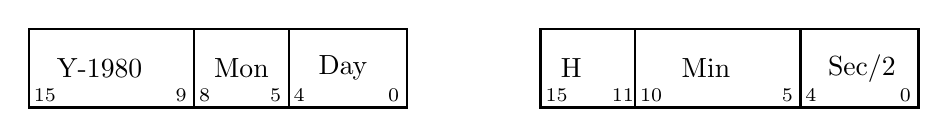
\begin{tikzpicture}
\tikzset{
    mylabel/.style={anchor=center},
    bitlabel/.style={font=\scriptsize,anchor=south west,inner sep=.5mm,text depth=.1mm},    
};
\begin{scope}[x=1.2cm]
\begin{scope}[thick]
    \draw (0, 0) rectangle (4, 1);
    \draw (0, 0) rectangle (1.75, 1);
    \node[bitlabel] at (0, 0) {15};
    \node[bitlabel] at (1.5, 0) {9};
    \draw (1.75, 0) rectangle (2.75, 1);
    \node[bitlabel] at (1.75, 0) {8};
    \node[bitlabel] at (2.5, 0) {5};
    \draw (2.75, 0) rectangle (4., 1);
    \node[bitlabel] at (2.75, 0) {4};
    \node[bitlabel] at (3.75, 0) {0};
\end{scope}
\node[mylabel] at (.75, 0.5) {Y-1980};
\node[mylabel] at (2.25, 0.5) {Mon};
\node[mylabel] at (3.325, 0.5) {Day};
\end{scope}

\begin{scope}[x=1.2cm,xshift=6.5cm]
\begin{scope}[thick]
    \draw (0, 0) rectangle (4, 1);
    \draw (0, 0) rectangle (1, 1);
    \node[bitlabel] at (0, 0) {15};
    \node[bitlabel] at (.7, 0) {11};
    \draw (1, 0) rectangle (2.75, 1);
    \node[bitlabel] at (1.0, 0) {10};
    \node[bitlabel] at (2.5, 0) {5};
    \draw (2.75, 0) rectangle (4., 1);
    \node[bitlabel] at (2.75, 0) {4};
    \node[bitlabel] at (3.75, 0) {0};
\end{scope}
\node[mylabel] at (.325, 0.5) {H};
\node[mylabel] at (1.75, 0.5) {Min};
\node[mylabel] at (3.4, 0.5) {Sec/2};
\end{scope}
\end{tikzpicture}
\begin{itemize}
    \item<2> Sec/2: 5 bits: range from 0--31
        \begin{itemize}
        \item corresponds to 0 to \textbf{62} seconds
        \end{itemize}
    \item<2> Vienna trick: set infected file times to \textbf{62} seconds
    \item<2> need to update times anyways --- hide tracks
\end{itemize}
\end{frame}

\section{more general virus choices}

\begin{frame}<1>[label=choices]{virus choices}
    \begin{itemize}
    \item \myemph<2>{where to put code}
    \item \myemph<3>{how to get code ran}
    \end{itemize}
\end{frame}

\section{problem 1: where to add code}

\againframe<2>{choices}

\begin{frame}{where to put code}
    \begin{itemize}
    \item considerations:
        \begin{itemize}
        \item spreading --- files that will be copied/reused
        \item spreading --- files that will be ran
        \item stealth --- user shouldn't know until too late
        \end{itemize}
    \end{itemize}
\end{frame}

\begin{frame}<1>[label=whereCode]{where to put code: options}
    \begin{itemize}
    \item one \textit{or more} of:
    \item \myemph<2>{replacing executable code}
    \item \myemph<3>{after executable code (Vienna)}
    \item \myemph<4>{in unused executable code}
    \item \myemph<5>{inside OS code}
    \item in memory
    \end{itemize}
\end{frame}

\subsection{replacing executable code}

\againframe<2>{whereCode}

\begin{frame}{replace executable}
    \begin{tikzpicture}
    \draw[thick] (0, 0) rectangle (4, -6) node[midway,align=center] {original\\executable};
    \draw[line width=2mm,-Latex,black!60] (4.1, -3) -- (6.9, -.5);
    \begin{scope}[xshift=7cm]
    \draw[thick,fill=red!20] (0, 0) rectangle (4, -1) node[midway,align=center] {virus code};
    \end{scope}
    \end{tikzpicture}
\end{frame}

\begin{frame}{replace executable?}
    \begin{itemize}
    \item seems silly --- not stealthy!
    \item has appeared in the wild --- ILOVEYOU
    \item 2000 ILOVEYOU Worm
        \begin{itemize}
        \item written in Visual Basic (!)
        \item spread via email
        \item replaced lots of files with copies of itself
        \end{itemize}
    \item huge impact --- because destroying data to copy itself
    \end{itemize}
\end{frame}

\begin{frame}{replace executable --- subtle}
    \begin{tikzpicture}
    \draw[thick] (0, 0) rectangle (4, -6) node[midway,align=center] {original\\executable};
    \draw[line width=2mm,-Latex,black!60] (4.1, -3) -- (6.9, -.5);
    \begin{scope}[xshift=7cm]
    \draw[thick,fill=red!20] (0, 0) rectangle (4, -1) node[midway,align=center] {virus code};
    \draw[thick,fill=yellow!20] (0, -1) rectangle (4, -1.5) node[midway,align=center,font=\scriptsize] {
        run original from tempfile
    };
    \draw[thick] (0, -1.5) rectangle (4, -7.2) node[midway,align=center] {original\\executable};
    \end{scope}
    \end{tikzpicture}
\end{frame}

\subsection{appending and compressing}

\againframe<3>{whereCode}

\begin{frame}{appending}
    \begin{tikzpicture}
    \draw[thick] (0, 0) rectangle (4, -5) node[midway,align=center] {original\\executable};
    \draw[line width=2mm,-Latex,black!60] (4.1, -3) -- (6.9, -3);
    \begin{scope}[xshift=7cm]
    \draw[thick] (0, 0) rectangle (4, -5) node[midway,align=center] {original\\executable};
    \draw[fill=red!20,thick] (0, -5) rectangle (4, -6)
        node[midway,align=center] {virus code};
    \draw[fill=red!20,thick] (0.5, -1) rectangle (1, -1.5);
    \node[anchor=west,red!50!black] at (1.25, -1.25) {jmp to virus};
    \draw[thick,Latex-] (1, -1.25) -- (1.4, -1.25);
    \end{scope}
    \end{tikzpicture}
\end{frame}

\begin{frame}{note about appending}
    \begin{itemize}
    \item COM files are very simple --- no metadata
    \item modern executable formats have length information to update
    \begin{itemize}
        \item add segment to program header
        \item update last segment of program header (size + make it executable)
    \end{itemize}
    \end{itemize}
\end{frame}

\begin{frame}{compressing viruses}
    \begin{itemize}
    \item file too big? how about \myemph{compression}
    \end{itemize}
    \begin{tikzpicture}
    \draw[thick] (0, 0) rectangle (4, -6) node[midway,align=center] {original\\executable};
    \draw[line width=2mm,-Latex,black!60] (4.1, -3) -- (6.9, -3);
    \begin{scope}[xshift=7cm]
    \draw[fill=red!20,thick] (0, 0) rectangle (4, -1) node[midway] {virus code};
    \draw[fill=red!20,thick] (0, -1) rectangle (4, -2) node[midway] {decompressor};
    \draw[pattern=north west lines,pattern color=black!70,thick] (0, -2) rectangle (4, -5)
        node[midway,fill=white,align=center] {compressed \\ executable};
    \draw[fill=black!60,thick] (0, -5) rectangle (4, -6)
        node[midway,white] {unused space};
    \end{scope}
    \end{tikzpicture}
\end{frame}

\subsection{cavities}

\againframe<4>{whereCode}

\begin{frame}{unused code???}
    \begin{itemize}
    \item why would a program have unused code????
    \end{itemize}
\end{frame}

\begin{frame}[fragile,label=lsStudy1]{unused code case study: /bin/ls}
    \begin{itemize}
    \item unreachable no-ops!
    \end{itemize}
\begin{Verbatim}[fontsize=\fontsize{9}{10}\selectfont,commandchars=Q\{\}]
...
  403788:	e9 59 0c 00 00       	jmpq   4043e6 <__sprintf_chk@plt+0x1a06>
  Qtextbf{40378d:	0f 1f 00             	nopl   (%rax)}
  403790:	ba 05 00 00 00       	mov    $0x5,%edx
...
  403ab9:	eb 4d                	jmp    403b08 <__sprintf_chk@plt+0x1128>
  Qtextbf{403abb:	0f 1f 44 00 00       	nopl   0x0(%rax,%rax,1)}
  403ac0:	4d 8b 7f 08          	mov    0x8(%r15),%r15
...
  404a01:	c3                   	retq   
  Qtextbf{404a02:	0f 1f 40 00          	nopl   0x0(%rax)}
  Qtextbf{404a06:	66 2e 0f 1f 84 00 00 	nopw   %cs:0x0(%rax,%rax,1)}
  Qtextbf{404a0d:	00 00 00 }
  404a10:	be 00 e6 61 00       	mov    $0x61e600,%esi
...
\end{Verbatim}
\end{frame}

\begin{frame}{why empty space?}
\begin{itemize}
\item Intel Optimization Reference Manual: \\
``\textbf{Assembly/Compiler Coding Rule 12. (M impact, H generality)} All branch targets should be 16-byte aligned.''
\begin{itemize}
    \item better for instruction cache {\small (and TLB and related caches)}
    \item better for instruction decode logic
    \item function calls count as branches for this purpose
\end{itemize}
\end{itemize}
\end{frame}

\begin{frame}{why weird nops}
    \begin{itemize}
    \item could fill with \myemph{anything} --- unreachable
    \item {\tt nop}s allow compiler/assembler to align \myemph{without checking reachability}
    \item {\tt nop}s better for \myemph{disassembly}
        \begin{itemize}
        \item Intel manual recommends form of {\tt nop} for different lengths
        \end{itemize}
    \item possibly \myemph{better for CPU}
        \begin{itemize}
        \item ``Placing data immediately following an indirect branch
              can cause performance problems. If the data consists of all zeros,
              it looks like a long stream of ADDs to memory destinations, and this can cause
              resource conflicts\ldots''
        \end{itemize}
    \end{itemize}
\end{frame}

\begin{frame}<1>[label=otherSpace]{other empty space}
\begin{itemize}
\item \myemph<2>{unused dynamic linking structure}
\item unused debugging/symbol table information?
\item unused space between segments
\item unused header space 
    \begin{itemize}
    \item file offsets of segments can be in middle of header
    \item loader doesn't care what segments ``mean''
    \end{itemize}
\end{itemize}
\end{frame}

\againframe<2>{otherSpace}

\begin{frame}[label=spaceDyn,fragile]{dynamic linking cavity}
\begin{itemize}
\item {\tt .dynamic} section --- data structure used by dynamic linker:
\item format: list of 8-byte type, 8-byte value
    \begin{itemize}
    \item terminated by type == 0 entry
    \end{itemize}
\end{itemize}
\begin{Verbatim}[fontsize=\fontsize{9}{10}\selectfont,commandchars=Q\{\}]
Contents of section .dynamic:
 600e28 01000000 00000000 01000000 00000000  ................
    Qtextit{... several non-empty entries ...}
 600f88 f0ffff6f 00000000 56034000 00000000  ...o....V.@.....
    Qtextit{VERSYM (required library version info at) 0x400356}
 600f98 Qtextit{00000000 00000000 00000000 00000000}  ................
    Qtextit{NULL --- end of linker info}
 600fa8 Qtextbf{00000000 00000000 00000000 00000000}  ................
    Qtextit{unused! (and below)}
 600fb8 Qtextbf{00000000 00000000 00000000 00000000}  ................
 600fc8 Qtextbf{00000000 00000000 00000000 00000000}  ................
 600fd8 Qtextbf{00000000 00000000 00000000 00000000}  ................
 600fe8 Qtextbf{00000000 00000000 00000000 00000000}  ................
\end{Verbatim}
\end{frame}

\begin{frame}{is there enough empty space?}
\begin{itemize}
    \item cavities look awfully small
    \item really small viruses?
    \item solution: chain cavities together
\end{itemize}
\end{frame}

\begin{frame}{case study: CIH (1)}
    \begin{tikzpicture}
    \draw[thick] (0, 0) rectangle (4, -6) node[midway,align=center] {original\\executable};
    \draw[line width=2mm,-Latex,black!60] (4.1, -3) -- (6.9, -3);
    \begin{scope}[xshift=7cm]
    \draw[fill=red!20,thick] (0, 0) rectangle (4, -0.5) node[midway] {virus startup code};
    \draw[fill=red!20,thick] (0, -0.5) rectangle (4, -1) node[midway] {virus code locs};
    \draw[thick] (0, -1) rectangle (4, -6);
    \draw[fill=red!20,thick] (0, -3) rectangle (4, -3.5)
        node[midway] {virus code part 1};
    \draw[fill=red!20,thick] (0, -4) rectangle (4, -4.5)
        node[midway] {virus code part 2};
    \draw[fill=red!20,thick] (0, -5) rectangle (4, -5.5)
        node[midway] {virus code part 3};
    \draw[dashed,thin,-Latex] (4, -0.75) -- (4.5, -0.75) |- (4, -3.25);
    \draw[dashed,thin,-Latex] (4, -0.75) -- (4.5, -0.75) |- (4, -4.25);
    \draw[dashed,thin,-Latex] (4, -0.75) -- (4.5, -0.75) |- (4, -5.25);
    \end{scope}
    \end{tikzpicture}
\end{frame}

\begin{frame}{case study: CIH (2)}
    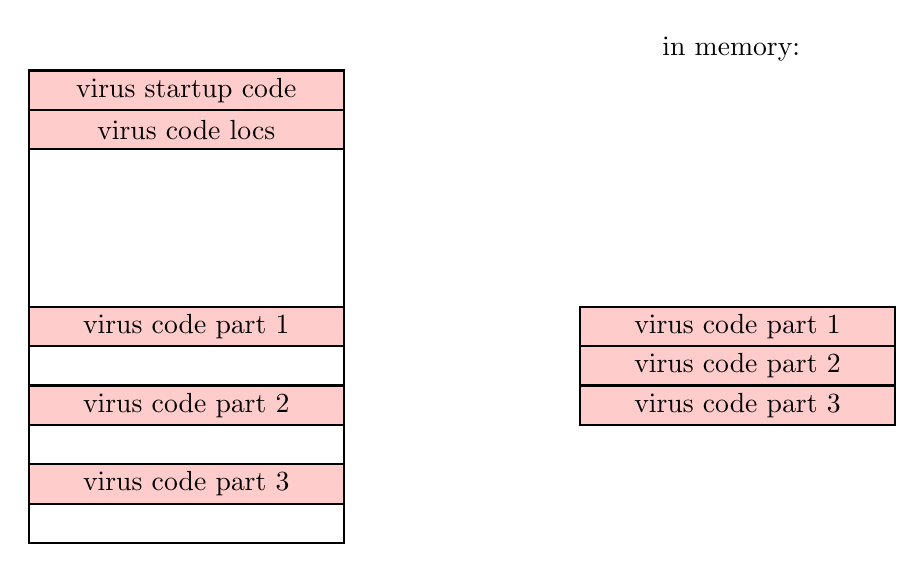
\begin{tikzpicture}
    \draw[fill=red!20,thick] (0, 0) rectangle (4, -0.5) node[midway] {virus startup code};
    \draw[fill=red!20,thick] (0, -0.5) rectangle (4, -1) node[midway] {virus code locs};
    \draw[thick] (0, -1) rectangle (4, -6);
    \draw[fill=red!20,thick] (0, -3) rectangle (4, -3.5)
        node[midway] {virus code part 1};
    \draw[fill=red!20,thick] (0, -4) rectangle (4, -4.5)
        node[midway] {virus code part 2};
    \draw[fill=red!20,thick] (0, -5) rectangle (4, -5.5)
        node[midway] {virus code part 3};
    \begin{scope}[xshift=7cm]
        \node[align=center,anchor=south] at (2, 0) { in memory: };
        \draw[fill=red!20,thick] (0, -3) rectangle (4, -3.5)
            node[midway] {virus code part 1};
        \draw[fill=red!20,thick] (0, -3.5) rectangle (4, -4)
            node[midway] {virus code part 2};
        \draw[fill=red!20,thick] (0, -4) rectangle (4, -4.5)
            node[midway] {virus code part 3};
    \end{scope}
    \end{tikzpicture}
\end{frame}

\begin{frame}{CIH cavities}
    \begin{itemize}
    \item gaps between sections
        \begin{itemize}
        \item common Windows linker \myemph{aligned} sections
        \item (align = start on address multiple of $N$, e.g. $4096$)
        \item probably means kilobytes of cavity in typical binary
        \item normal Linux linker doesn't do this
        \begin{itemize}\item smaller executables but less convenient for linker+loader\end{itemize}
        \end{itemize}
    \item reassembling: unsplit multibyte instructions
    \end{itemize}
\end{frame}

\subsubsection{special cavity: relocation section (PE)}

\subsection{boot sectors}

\againframe<5>{whereCode}

\begin{frame}<1-2>[label=bootProc]{boot process}
    \begin{tikzpicture}
        \begin{scope}[start chain=going below,every node/.style={draw,align=center,join,on chain,thick,minimum width=3.5cm},
                      every join/.style={-Latex,thick}]
        \node[draw=none] (fixedLoc) { processor reset };
        \node[alt=<3>{draw=red,very thick}{}] (bios) {BIOS/EFI \\ \small (chip on motherboard)};
        \node[alt=<2>{draw=red,very thick}{}] (bootloader) {bootloader};
        \node[alt=<4>{draw=red,very thick}{}] (os) {operating system};
        \end{scope}
        \node[left=.5cm of bios,font=\small] (biosLabel) {very CPU/motherboard-specific code};
        \draw[-Latex,thick] (biosLabel) -- (bios);
        \node[left=.5cm of bootloader,font=\small,align=right] (bootloaderLabel) {fixed location on disk \\ code that understands files};
        \draw[-Latex,thick] (bootloaderLabel) -- (bootloader);
        \node[left=.5cm of os,font=\small] (osLabel) {files in a filesystem};
        \draw[-Latex,thick] (osLabel) -- (os);
    \end{tikzpicture}
\end{frame}

\begin{frame}{bootloaders in the DOS era}
    \begin{itemize}
    \item used to be common to boot from floppies
    \item \myemph{default to booting from floppy} if present
        \begin{itemize}
        \item even if hard drive to boot from
        \end{itemize}
    \item applications distributed as bootable floppies
    \item so bootloaders on all devices were a target for viruses
    \end{itemize}
\end{frame}

\begin{frame}{historic bootloader layout}
    \begin{itemize}
    \item bootloader in \myemph{first sector} (512 bytes) of device
    \item (along with partition information)
    \item code in BIOS to copy bootloader into RAM, start running
    \item bootloader responsible for disk I/O etc.
        \begin{itemize}
        \item some library-like functionality in BIOS for I/O
        \end{itemize}
    \end{itemize}
\end{frame}

\begin{frame}{bootloader viruses}
    \newcommand{\tearBox}{
        \draw[very thick] (0, -6) -- (0, 0) -- (4, 0) -- (4, -6);
        \draw[thick] (0, -6) -- (1.2, -5.5) -- (2., -6.6) -- (2.6, -5.8) -- (3.5, -6.6) -- (4, -6);
    }
    \begin{itemize}
    \item example: Stoned
    \end{itemize}
    \begin{tikzpicture}
        \draw[fill=green!20] (0, 0) rectangle (4, -.2);
        \draw[fill=yellow!20] (0, -.2) rectangle (4, -0.5) node[midway,font=\tiny] { partition table };
        \draw[fill=green!20] (0, -.5) rectangle (4, -1.0) node[midway,font=\small] { bootloader };
        \tearBox
        \begin{scope}[xshift=7cm]
        \draw[fill=red!20] (0, 0) rectangle (4, -.2);
        \draw[fill=yellow!20] (0, -.2) rectangle (4, -0.5) node[midway,font=\tiny] { partition table };
        \draw[fill=red!20] (0, -.5) rectangle (4, -1.0) node[midway,font=\small] { virus code };
        \begin{scope}[yshift=-4cm]
        \draw[fill=green!20] (0, 0) rectangle (4, -.2);
        \draw[fill=green!20] (0, -.5) rectangle (4, -1.0) node[midway,font=\small] { saved bootloader };
        \draw[dashed,fill=yellow!20] (0, -.2) rectangle (4, -0.5) node[midway,font=\tiny] { partition table (unused) };
        \end{scope}
        \tearBox 
        \end{scope}
        \draw[line width=1mm,black!50, -Latex] (4.2, -3) -- (6.8, -3);

        \begin{pgfonlayer}{bg}
            \begin{visibleenv}<2>
                \path[fill=blue!30] (0, -4) rectangle (4, -5) node[midway] { data here??? };
            \end{visibleenv}
        \end{pgfonlayer}
    \end{tikzpicture}
\end{frame}

\begin{frame}{data here???}
    \begin{itemize}
        \item might be data there --- risk
        \item some unused space after partition table/boot loader common
            \begin{itemize}
            \item (allegedly)
            \end{itemize}
        \item also be filesystem metadata not used on smaller floppies/disks
        \vspace{.5cm}
        \item but could be wrong --- oops
    \end{itemize}
\end{frame}

\begin{frame}{modern bootloaders --- UEFI}
    \begin{itemize}
    \item BIOS-based boot is going away (slowly)
    \item new thing: UEFI (Universal Extensible Firmware Interface)
    \item like BIOS:
        \begin{itemize}
        \item library functionality for bootloaders
        \item loads initial code from disk/DVD/etc.
        \end{itemize}
    \item unlike BIOS:
        \begin{itemize}
        \item much more understanding of file systems
        \item much more modern set of library calls
        \end{itemize}
    \end{itemize}
\end{frame}

\begin{frame}{modern bootloaders --- secure boot}
    \begin{itemize}
    \item ``Secure Boot'' is a common feature of modern bootloaders
    \item idea: UEFI/BIOS code checks bootloader code, fails if not okay
        \begin{itemize}
        \item requires user intervention to use not-okay code
        \end{itemize}
    \end{itemize}
\end{frame}

\begin{frame}{Secure Boot and keys}
    \begin{itemize}
    \item Secure Boot relies on cryptographic signatures
        \begin{itemize}
        \item idea: accept only ``legitimate'' bootloaders
        \item legitimate: known authority vouched for them
        \end{itemize}
    \item user control of their own systems?
        \begin{itemize}
        \item in theory: can add own keys
        \end{itemize}
    \item what about changing OS instead of bootloader?
        \begin{itemize}
        \item need smart bootloader
        \end{itemize}
    \end{itemize}
\end{frame}

\againframe<3>{bootProc}

\begin{frame}{BIOS/UEFI implants}
    \begin{itemize}
    \item infrequent
    \item BIOS/UEFI code is \myemph{very non-portable}
    \item BIOS/UEFI update may require physical access
    \item BIOS/UEFI code may require cryptographic signatures
    \item \ldots but \myemph{very hard to remove} --- ``persist'' other malware
    \item reports of BIOS/UEFI-infecting ``implants''
        \begin{itemize}
        \item sold by Hacking Team (Milan-based malware company) 
        \item listed in leaked NSA Tailored Access Group catalog
        \end{itemize}
    \end{itemize}
\end{frame}

\againframe<4>{bootProc}

\begin{frame}{system files}
    \begin{itemize}
    \item simpliest strategy: stuff that runs when you start your computer
    \item add a new startup program, run in the background
        \begin{itemize}
        \item easy to blend in
        \end{itemize}
    \vspace{.5cm}
    \item alternatively, infect one of many system programs automatically run
    \end{itemize}

    % FIXME: example from CodeRed or similar?
\end{frame}

\begin{frame}{memory residence}
    \begin{itemize}
    \item malware wants to keep doing stuff
    \item one option --- background process (easy on modern OSs)
    \item also stealthy options:
        \begin{itemize}
        \item insert self into OS code
        \item insert self into other running programs
        \end{itemize}
    \item more commonly, OS code used for hiding malware
        \begin{itemize}
        \item topic for later
        \end{itemize}
    \end{itemize}
\end{frame}

\begin{frame}{}
\end{frame}

% FIXME: some rootkit example
\section{problem 2: where to invoke code}

\againframe<3>{choices}

\begin{frame}<1-2>[label=invokeOptions]{invoking virus code: options}
    \begin{itemize}
    \item boot loader
    \item \myemph<2>{change starting location} 
    \item alternative approaches: ``entry point obscuring''
    \item \myemph<3>{edit code that's going to run anyways}
    \item \myemph<4>{replace a function pointer} (or similar)
    \item \ldots
    \end{itemize}
\end{frame}

\subsection{start location}

\begin{frame}[fragile,label=invokeStarting]{starting locations}
\begin{Verbatim}[fontsize=\fontsize{10}{11}\selectfont,commandchars=Q\{\}]
/bin/ls:     file format elf64-x86-64
/bin/ls
architecture: i386:x86-64, flags 0x00000112:
EXEC_P, HAS_SYMS, D_PAGED
start address Qmyemph{0x00000000004049a0}
\end{Verbatim}
    \begin{itemize}
    \item modern executable formats have `starting address' field
    \item just change it, insert jump to old address after virus code
    \end{itemize}
\end{frame}

\againframe<3>{invokeOptions}

\subsection{code run anyways}

\subsubsection{at natural entry point}

\begin{frame}[fragile,label=runAnyways]{run anyways?}
    \begin{itemize}
    \item add code at start of program (Vienna)
    \item return with padding after it:
\begin{Verbatim}[fontsize=\fontsize{10}{11}\selectfont,commandchars=Q\{\}]
  404a01:       c3                      Qtextbf{retq}
  404a02:       0f 1f 40 00             nopl   0x0(%rax)
                Qtextit{replace with}
  404a01:       e9 XX XX XX XX          Qtextbf{jmpq    YYYYYYY}
\end{Verbatim}
    \item any random place in program?
        \begin{itemize}
        \item just not in the \myemph{middle of instruction}
        \end{itemize}
    \end{itemize}
\end{frame}

\subsubsection{other locations: challenge}

\begin{frame}[fragile,label=findValidChallenge]{challenge: valid locations}
    \begin{itemize}
    \item x86: probably don't want a full instruction parser
    \item x86: might be non-instruction stuff mixed in with code:
\begin{lstlisting}[language=myasm,style=smaller]
do_some_floating_point_stuff:
            movss float_one(%rip), %xmm0
            ...
            retq
float_one: .float 1
\end{lstlisting}
    \begin{itemize}
        \item floating point value one ({\tt 00 00 80 3f}) is not valid machine code
        \item disassembler might lose track of instruction boundaries
    \end{itemize}
    \end{itemize}
\end{frame}

\subsubsection{function calls}

\begin{frame}[fragile,label=findValidFindFunc]{finding function calls}
    \begin{itemize}
    \item one idea: replace calls
    \item normal x86 call FOO: {\tt E8 \textit{(32-bit value: PC - address of foo)}}
    \item could look for E8 in code --- \myemph{lots of false positives}
        \begin{itemize}
        \item probably even if one excludes out-of-range addresses
        \end{itemize}
    \end{itemize}
\end{frame}

\begin{frame}[fragile,label=findValidFindFunc2]{really finding function calls}
\lstset{language=myasm,style=small}
    \begin{itemize}
    \item e.g. some popular compilers started x86-32 functions with
\begin{lstlisting}
foo:
    push %ebp       // push old frame pointer
    // 0x55
    mov %esp, %ebp  // set frame pointer to stack pointer
    // 0x89 0xec
\end{lstlisting}
    \item use to identify when {\tt e8} refers to real function
    \begin{itemize}
    \item (full version: also have some other function start patterns)
    \end{itemize}
    \end{itemize}
\end{frame}

\subsubsection{linker stubs}

\begin{frame}[fragile,label=stubReplace]{remember stubs?}
\begin{Verbatim}[commandchars=Q\{\},fontsize=\fontsize{8}{9}\selectfont]
0000000000400400 <puts@plt>:
  400400:	ff 25 12 0c 20 00    	jmpq   *0x200c12(%rip) 
                    /* 0x200c12+RIP = _GLOBAL_OFFSET_TABLE_+0x18 */
  400406:	68 00 00 00 00       	pushq  $0x0
  40040b:	e9 e0 ff ff ff       	jmpq   4003f0 <_init+0x28>
    Qtextbf{ replace with: }
  400400:	e8 XX XX XX XX          Qtextbf{jmpq virus_code}
  400405:       90                      nop
  400406:	68 00 00 00 00       	pushq  $0x0
  40040b:	e9 e0 ff ff ff       	jmpq   4003f0 <_init+0x28>
\end{Verbatim}
\begin{itemize}
    \item in known location (particular section of executable)
\end{itemize}
\end{frame}


\subsection{replacing pointers}

\againframe<4>{invokeOptions}

\begin{frame}[fragile,label=stubsReplacePtr]{stubs again}
\begin{Verbatim}[commandchars=Q\{\},fontsize=\fontsize{8}{9}\selectfont]
0000000000400400 <puts@plt>:
  400400:	ff 25 12 0c 20 00    	jmpq   Qtextbf{*0x200c12(%rip)}
                    /* 0x200c12+RIP = Qtextbf{_GLOBAL_OFFSET_TABLE_+0x18} */
  400406:	68 00 00 00 00       	pushq  $0x0
  40040b:	e9 e0 ff ff ff       	jmpq   4003f0 <_init+0x28>
\end{Verbatim}
\begin{itemize}
\item don't edit stub --- edit initial value of {\tt \_GLOBAL\_OFFSET\_TABLE}
    \begin{itemize}
    \item stored in data section of executable
    \end{itemize}
\item originally: pointer {\tt 0x400406}; new --- virus code
\end{itemize}
\end{frame}

\begin{frame}[fragile,label=relocReplace]{relocations?}
\begin{Verbatim}[commandchars=Q\{\},fontsize=\fontsize{8}{9}\selectfont]
hello.exe:     file format elf64-x86-64

DYNAMIC RELOCATION RECORDS
OFFSET           TYPE              VALUE 
0000000000600ff8 R_X86_64_GLOB_DAT  __gmon_start__
0000000000601018 R_X86_64_JUMP_SLOT  Qtextit{puts@GLIBC_2.2.5}
    Qtextbf{replace with:}
0000000000601018 R_X86_64_JUMP_SLOT  Qtextbf{_start + offset_of_virus}
0000000000601020 R_X86_64_JUMP_SLOT  __libc_start_main@GLIBC_2.2.5
\end{Verbatim}
\begin{itemize}
    \item<1> tricky --- usually no symbols from executable in dynamic symbol table
        \begin{itemize}
        \item (symbols from debugger/disassembler are a different table)
        \item Linux --- need to link with {\tt -rdynamic}
        \end{itemize}
    \item<2> but\ldots same idea works on shared library itself
\end{itemize}
\end{frame}

\begin{frame}{infecting shared libraries}
\begin{tikzpicture}
    \draw[thick] (0, 0) rectangle (4, -6) coordinate (bottomRight) node[midway] { \tt kernel32.dll };
    \draw[thick,fill=yellow!20] (0, 0) rectangle (4, -0.5) node[midway,font=\small] {header};
    \draw[thick,fill=blue!20] (0, -0.5) rectangle (4, -2.0);
    \node[font=\small,anchor=north] at (2, -0.5) {symbol table};
    \node[anchor=north west,font=\fontsize{9}{10}\selectfont] (GFAName) at (0, -0.9) {
        \tt GetFileAttributesA
    };
    \node[anchor=north west] at (GFAName.south west) {\tt \ldots};
    \draw[-Latex,thick] ([xshift=.5mm]GFAName.east) coordinate (startArrowA) -- ([xshift=.5cm]GFAName.west -| bottomRight) |- (3, -5);
    \fill[black] (startArrowA) circle[radius=.5mm];

    \draw[line width=2mm,-Latex,black!60] (4.6, -3) -- (6.9, -3);
    \begin{scope}[xshift=7cm]
    \draw[thick] (0, 0) rectangle (4, -6) coordinate (bottomRight) node[midway] { \tt kernel32.dll };
    \draw[thick,fill=yellow!20] (0, 0) rectangle (4, -0.5) node[midway,font=\small] {header};
    \draw[thick,fill=blue!20] (0, -0.5) rectangle (4, -2.0);
    \node[font=\small,anchor=north] at (2, -0.5) {symbol table};
    \draw[thick,fill=red!20] (0, -6) rectangle (4, -7) node[midway,font=\small] {virus code};
    \node[anchor=north west,font=\fontsize{9}{10}\selectfont] (GFANameB) at (0, -0.9) {
        \tt GetFileAttributesA
    };
    \node[anchor=north west] at (GFANameB.south west) {\tt \ldots};
    \draw[-Latex,very thick,red] ([xshift=.5mm]GFANameB.east) coordinate (startArrowA) -- ([xshift=.5cm]GFANameB.west -| bottomRight) |- (1, -6.2);
    \fill[red] (startArrowA) circle[radius=.5mm];
    \end{scope}
\end{tikzpicture}
\end{frame}


\begin{frame}{summary}
    \begin{itemize}
    \item how to hide:
        \begin{itemize}
        \item separate executable
        \item append
        \item existing ``unused'' space
        \item compression
        \end{itemize}
    \item how to run:
        \begin{itemize}
        \item change entry point
        \item or ``entry point obscuring'':
        \item change some code (requires care!)
        \item change library
        \end{itemize}
    \end{itemize}
\end{frame}

\begin{frame}{anti-malware strategies}
    \begin{itemize}
    \item antivirus goals:
    \begin{itemize}
    \item prevent malware from running
    \item prevent malware from spreading
    \item undo the effects of malware
    \end{itemize}
    \end{itemize}
\end{frame}

\begin{frame}{malware detection}
    \begin{itemize}
    \item important part: detecting malware
    \item simple way:
        \begin{itemize}
        \item have a copy of a malicious execu\tikzmark{exec}table
        \item compare every\tikzmark{every} program to it
        \end{itemize}
    \end{itemize}
    \begin{tikzpicture}[overlay, remember picture]
        \coordinate (overlayLoc) at ([yshift=-1cm]current page.center);
        \begin{visibleenv}<2>
            \node[mycallout=exec,anchor=center] at (overlayLoc) {
                how big? every executable infected with every virus?
            };
        \end{visibleenv}
        \begin{visibleenv}<3>
            \node[mycallout=every,anchor=center] at (overlayLoc) {
                when? how fast?
            };
        \end{visibleenv}
    \end{tikzpicture}
\end{frame}

\section{signature-based detection}

\begin{frame}{malware ``signatures''}
    \begin{itemize}
    \item antivirus vendor have ``signatures'' for known malware
    \item many options to represent signatures
    \item thought process: signature for Vienna?
    \end{itemize}
\end{frame}

\begin{frame}[fragile,label=viennaSigs]{exercise: signatures for Vienna}
\lstset{language=myasm,style=small}
\begin{tabular}{lll}
\begin{lstlisting}
jmp 0x0700
mov $0x9e4e, %si
...
push %cx
mov $0x8f9, %si
...
mov $0x0100, %di
mov $3, %cx
rep movsb
...
\end{lstlisting}
&
\begin{lstlisting}
...
add $0x2f9, %cx
mov %si, %di
sub $0x1f7, %di
mov %cx, (%di)
...
mov $0x288, %cx
mov $0x40 %ah
mov $si, $dx
sub $0x1f9, %dx
int 0x21
...
\end{lstlisting}
&
\begin{lstlisting}
pop %cx
xor %ax, %ax
xor %bx, %bx
xor %dx, %dx
mov $0x0100 %di
push %di
xor %di, %di
ret
\end{lstlisting}
\\
\end{tabular}
\end{frame}

\begin{frame}{simple signature}
    \begin{itemize}
    \item all the code Vienna copies
    \item \ldots{} except changed {\tt mov} to {\tt \%si}
    \vspace{.5cm}
    \item virus doesn't change it to relocate
    \item includes infection code --- definitely malicious
    \end{itemize}
\end{frame}

\begin{frame}{signature generality}
    \begin{itemize}
    \item the Vienna virus was copied a bunch of times
    \item small changes, ``payloads'' added
        \begin{itemize}
        \item print messages, do malicious things, \ldots
        \end{itemize}
    \item this signature will not detect any variants
    \item can we do better?
    \end{itemize}
\end{frame}

\begin{frame}{simple signature (2)}
    \begin{itemize}
    \item Vienna infection code
        \begin{itemize}
        \item scans directory, finds files
        \end{itemize}
    \item likely to stay the same in variants\ldots
    \item \ldots except that virus writer's will change it
    \end{itemize}
\end{frame}

{ % all template changes are local to this group.
    \setbeamertemplate{navigation symbols}{}
    \contourlength{.2mm}
    \begin{frame}[plain]
        \begin{tikzpicture}[remember picture,overlay]
            \node[at=(current page.center)] {
                
\includegraphics[width=\paperwidth]{1600x1200-Tom-Jerry-Chase}
            };
            %\draw[help lines] (0, 0) grid (12, -8);
            \node[cross out,draw,line width=1mm,black,at={(9,-6)},anchor=center,minimum width=6cm,minimum height=1.25cm] {};
            \node[at={(3,-8.25)},anchor=center,font=\Huge\bfseries,
                red,align=left] {\contour{black}{Anti-\hspace{-.4ex}Virus}};
            \node[at={(6.5,-8.25)},anchor=center,font=\large\bfseries,
                red,align=left,rotate=30] {\contour{black}{and}};
            \node[at={(8.5,-8.25)},anchor=center,font=\Huge\bfseries,
                red,align=left] {\contour{black}{Virus}};
        \end{tikzpicture}
     \end{frame}
}
\begin{frame}{signature checking}
    \begin{itemize}
    \item how fast is signature checking?
    \item clever trick: only read end of file (where virus code will be)
    \item very fast
    \end{itemize}
\end{frame}

\begin{frame}{generalizing the signature}
    \begin{itemize}
    \item another possibility: detect writing to {\tt 0x100}
    \item {\tt 0x100} was DOS program entry code  --- no program should do this
    \item problem: how to represent this
    \end{itemize}
\end{frame}

\begin{frame}{regular expressions}
    \begin{itemize}
    \item one method of representing patterns like this: \\
          regular expressions (regexes)
    \item restricted language allows very fast implementations
        \begin{itemize}
        \item especially when there's a long list of patterns to look for
        \end{itemize}
    \item homework assignment next week
    \item more next class
    \item along with other anti-virus techniques
    \end{itemize}
\end{frame}

\begin{frame}{anti-virus: essential or worthless?}
    \begin{itemize}
    \item ungraded homework assignment
    \item watch Hanno B\"ock's talk ``In Search of Evidence-Based IT Security''
    \item a rant mostly about antivirus-like software
    \end{itemize}
\end{frame}


\section{Backup Slides}

\begin{frame}{Case Study: Vienna Virus}
\begin{itemize}
    \item Vienna: virus from the 1980s
    \item This version: published in Ralf Burger, ``Computer Viruses: a high-tech disease'' (1988)
    \item targetted COM-format executables on DOS
\end{itemize}
\end{frame}

\begin{frame}{Diversion: .COM files}
    \begin{itemize}
    \item .COM is a \myemph{very simple} executable format
    \item no header, no segments, no sections
    \item file contents loaded at fixed address {\tt 0x0100}
    \item execution starts at {\tt 0x0100}
    \item everything is read/write/execute (no virtual memory)
    \end{itemize}
\end{frame}

\subsection{Vienna: entry/exit}

\begin{frame}[fragile,label=vienna]{Vienna: infection}
\lstset{
    language=myasm,
    style=smaller
}
\begin{tikzpicture}
\tikzset{programBox/.style={draw,thick},every label/.style={inner sep=1mm,outer sep=0mm,overlay}}
\node[programBox,minimum height=3cm,label={north:uninfected},anchor=north west] (uninfect) at (0,0) {
\begin{lstlisting}
0x0100:
    mov $0x4f28, %cx
    /* b9 28 4f */
0x0103:
    mov $0x9e4e, %si
    /* be 4e 9e */
    mov %si, %di
    push %ds
    /* more normal
       program
       code */
....
0x0700: /* end */

\end{lstlisting}
};
\node[programBox,anchor=north west,label={north:infected}] at ([xshift=1cm]uninfect.north east) {
\begin{lstlisting}
0x0100: jmp 0x0700
0x0103: mov $0x9e4e, %si
...
0x0700:
    push %cx
    ... // %si <- 0x903
    mov $0x100, %di
    mov $3, %cx
    rep movsb
    ...
    mov $0x0100, %di
    push %di
    xor %di, %di
    ret
...
0x0903:
    .bytes 0xb9 0x28 0x4f
...
\end{lstlisting}
};
\end{tikzpicture}
\end{frame}

\begin{frame}[fragile,label=viennaFixup]{Vienna: ``fixup''}
\lstset{
    language=myasm,
    style=small,
    moredelim={**[is][\btHL<2>]{~hi2~}{~endhi2~}},
    moredelim={**[is][\btHL<3>]{~hi3~}{~endhi3~}},
}
\begin{lstlisting}
0x0700:
    push %cx // initial value of %cx matters??
    mov ~hi3~$0x8fd~endhi3~, %si // %si <- beginning of data
    mov %si, %dx // save %si
        // movsb uses %si, so
        // can't use another register
    add $0xa, %si // offset of saved code in data
    mov $0x100, %di // target address
    mov $3, %cx // bytes changed
    /* copy %cx bytes from (%si) to (%di) */
    rep movsb 
    ...
...
// saved copy of original application code
0x903: ~hi2~.byte 0xb9 .byte 0x28 .byte 0x4f~endhi2~
\end{lstlisting}
\end{frame}

\begin{frame}[fragile,label=viennaReturn]{Vienna: return}
\lstset{language=myasm,style=small}
\begin{lstlisting}
0x08e7:
    pop %cx // restore initial value of %cx, %sp
    xor %ax, %ax // %ax <- 0
    xor %bx, %bx
    xor %dx, %dx
    xor %si, %si
    // push 0x0100
    mov $0x0100, %di
    push %di 
    xor %di, %di // %di <- 0
    // pop 0x0100 from stack
    // jmp to 0x0100
    ret 
\end{lstlisting}
\begin{itemize}
\item<1> question: why not just jmp 0x0100 ?
\end{itemize}
\end{frame}

\subsection{Vienna: replicate}

\begin{frame}<1>[label=viennaOutline]{Vienna: infection outline}
\begin{itemize}
\item Vienna \myemph{appends} code to infected application
\vspace{.5cm}
\item \myemph<2>{where does it read the code come from?}
\item \myemph<3>{how is code adjusted for new location in the binary?}
    \begin{itemize}\item what linker would do\end{itemize}
\item \myemph<4>{how does it keep files from getting infinitely long?}
\end{itemize}
\end{frame}

\againframe<2>{viennaOutline}

\begin{frame}{quines}
\begin{itemize}
    \item exercise: write a C program that outputs its source code
        \begin{itemize}
        \item (pseudo-code only okay)
        \end{itemize}
    \item possible in any {\small (Turing-complete)} programming language
    \item called a ``quine''
\end{itemize}
\end{frame}

\begin{frame}[fragile,label=quineClever]{clever quine solution}
\lstset{language=C,style=small,
    moredelim={**[is][\btHL<2|handout:0>]{@hi2@}{@endhi@}},
    moredelim={**[is][\btHL<3|handout:0>]{@hi3@}{@endhi@}},
    showstringspaces=false,
}
\begin{lstlisting}
#include <stdio.h>
char*x="int main(){
       `\btHL<2>{printf(p,10,34,x,34,10,34,p,34,10,x,10);}`
       }";
@hi3@char*p@endhi@="#include <stdio.h>%c
    char*x=%c%s%c;%cchar*p=%c%s%c;
    %c%s%c";
int main(){
    @hi2@printf(p,10,34,x,34,10,34,p,34,10,x,10);@endhi@
}
\end{lstlisting}
\begin{itemize}
\item some line wrapping for readability --- shouldn't be in actual quine
\end{itemize}
\begin{tikzpicture}[overlay,remember picture]
    \begin{visibleenv}<2|handout:0>
        \node[fill=white,draw,thick,align=left] at (current page.center) {
            {\tt printf} to fill template: \\
            {\tt 10} = newline; {\tt 34} = double-quote; \\
            {\tt x}, {\tt p} = template/constant strings
        };
    \end{visibleenv}
    \begin{visibleenv}<3|handout:0>
        \node[fill=white,draw,thick,align=left] at ([yshift=1cm]current page.center) {
            template filled by printf
        };
    \end{visibleenv}
\end{tikzpicture}
\end{frame}

\begin{frame}[fragile,label=quineDumb]{dumb quine solution}
\begin{lstlisting}[language=C,style=small]
#include <stdio.h>
int main(void) {
    char buffer[1024];
    FILE *f = fopen("quine.c", "r");
    size_t bytes = fread(buffer, 1,
                         sizeof(buffer), f);
    fwrite(buffer, 1, bytes, stdout);
    return 0;
}
\end{lstlisting}
\begin{itemize}
\item a lot more straightforward!
\item but ``cheating''
\end{itemize}
\end{frame}

\begin{frame}[fragile,label=virusWriting]{Vienna copying}
\lstset{
    style=small,
    language=myasm,
    moredelim={**[is][\btHL<2|handout:0>]{@hi2@}{@endhi@}},
}
\begin{lstlisting}
@hi2@mov $0x8f9, %si@endhi@ // %si = beginning of virus data
...
mov $0x288, %cx // length of virus
mov $0x40, %ah  // system call # for write
mov %si, %dx
sub $0x1f9, %dx // %dx = beginning of virus code
int 0x21 // make write system call
\end{lstlisting}
\end{frame}

\begin{frame}{32-bit ModRM table}
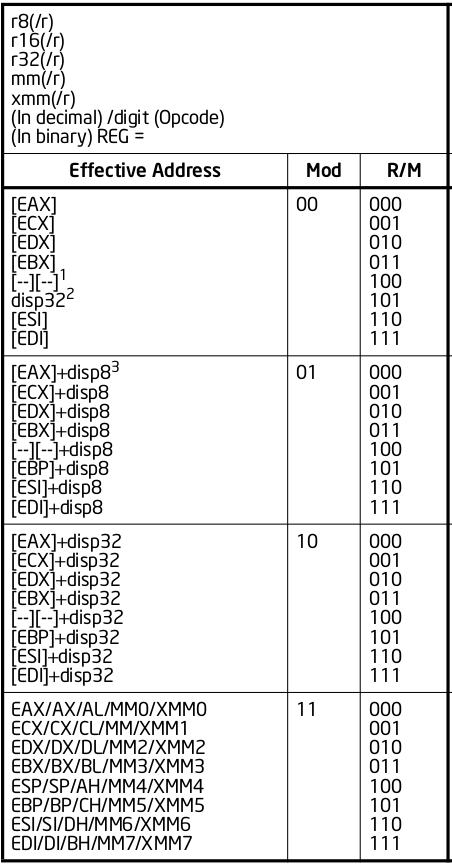
\includegraphics[height=0.8\textheight]{32bitmodrm}
\end{frame}

\begin{frame}{SIB table}
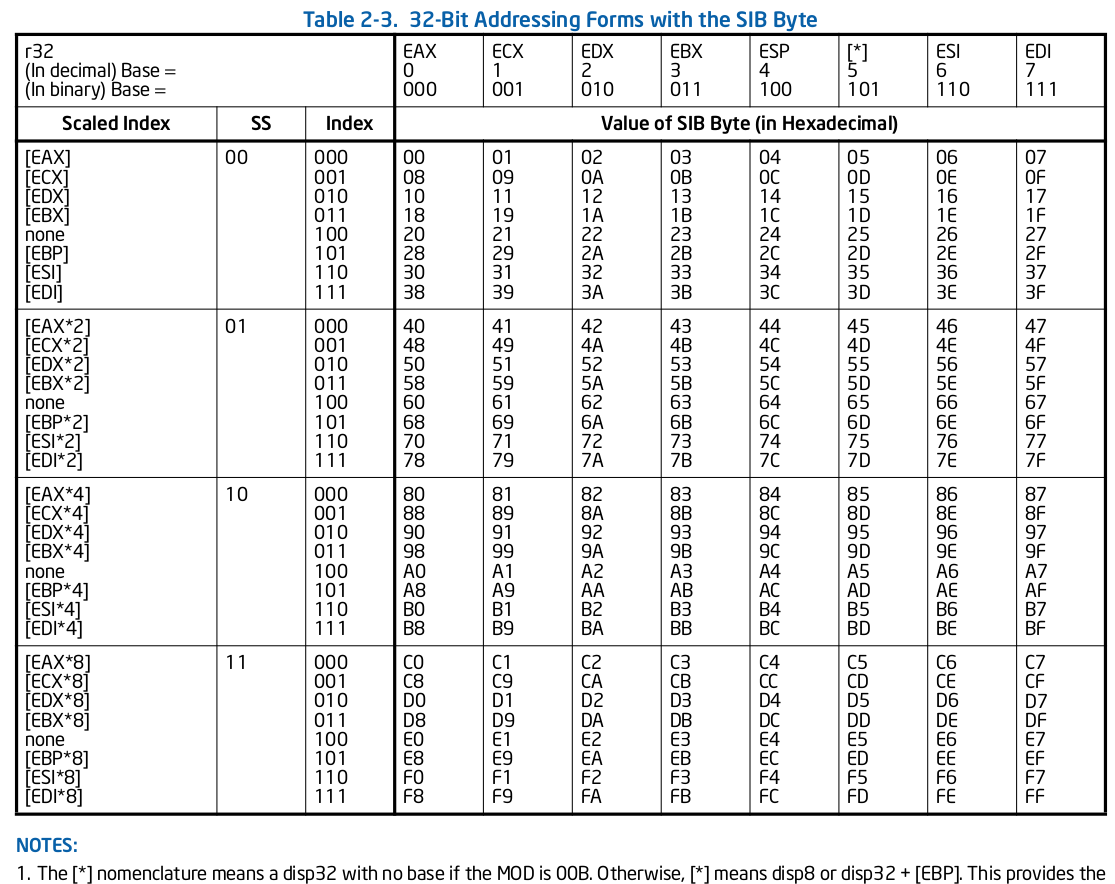
\includegraphics[height=0.8\textheight]{32bitsib}
\end{frame}
